\subsection{Nodes and Edges} \label{subsec:nodes_and_edges}

As a next step we focus on describing how to create the base information for our advanced PPI Network.
The graph database contains gene and protein node types.
The Edges between the proteins build a classical PPI Network and are called Interactions. % mehr biologische Erklärung?
The second type of Edges, called Connections, are the Link between Proteins and Genes.
As Shown in the Figure \ref{fig:03_02_Network}.
% TODO Wir machen das, weil …

\begin{figure}[h]
\centering
\includegraphics[width=0.8\textwidth]{figures/03_02_Network}
\caption{Schema of the Graph Database}
\label{fig:03_02_Network}
\end{figure}

For each of those 4 components we will create a table that will serve as base for creating the graph database.\\


For creating the \textbf{gene nodes} we need to use the preprocessed CMP and GTEx datasets,
which contain mean TPM values for cancerous and healthy genes.
We build the intersection of both datasets on their ENS ID to get a subset that only contains genes with TPM values for both conditions.
% filtering for genes that have a gene-protein connection
To fulfill our first objective \ref{obj:delta_tpm},
we need to calculate a measure that captures significant changes between cancerous and healthy gene activity.
When examining the mean TPM values per dataset, we observe a right-skewed distribution, with most values close to zero
and a long tail extending towards higher values.
The cancerous TPM values vary from 0 to approximately 41.173, while the healthy TPM values range from 0 to around 36.200.



To normalize the TPM values from both datasets and enable better comparability, we perform a common log scaling between 0 and 1 for all TPM values combined.

\begin{equation}
\label{eq:tpm_normalization}
f(x) = \frac{\log(1 + x) - \log(1 + x_{min})}{\log(1 + x_{max}) - \log(1 + x_{min})}
\end{equation}
% TODO Naming log_norm(x) - entsptechend Funktion im Code anpassen

where $x_{max}$ and $x_{min}$ are the maximum and minimum TPM values across both datasets.
After applying the normalization, the distribution of the TPM values is more balanced, as shown in Figure \ref{fig:03_02_normalized_tpm_both}.

%TODO Bilder nebeneinander
\begin{figure}[h]
    \centering
    \subfigure[Histogram of TPM Values of GTEx Dataset]{
       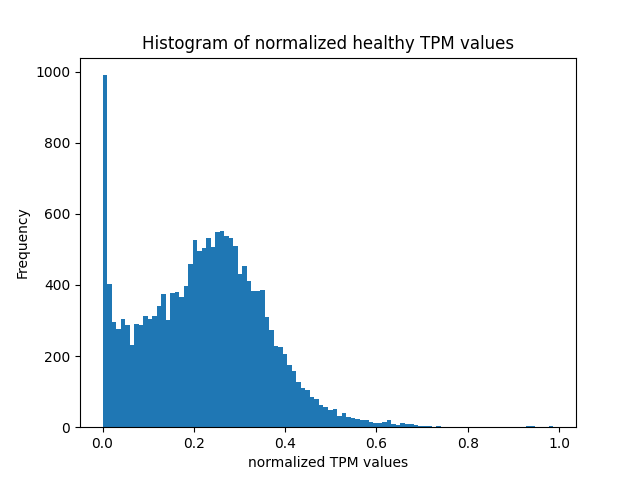
\includegraphics[width=0.45\textwidth]{figures/03_02_normalized_gtex_tpm}
        \label{fig:03_02_normalized_tpm_gtex}
    }
    \caption{Comparison of TPM Values from CMP and GTEx Datasets}
    \hfill
    \subfigure[Histogram of TPM Values of CMP Dataset]{
       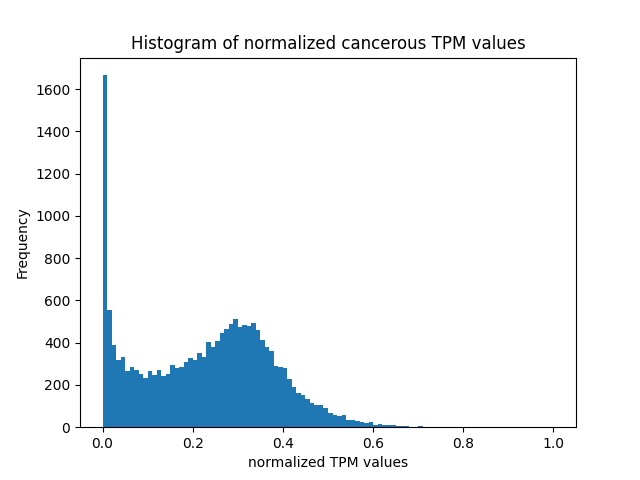
\includegraphics[width=0.45\textwidth]{figures/03_02_normalized_cmp_tpm}
        \label{fig:03_02_normalized_tpm_cmp}
    }
    \label{fig:03_02_normalized_tpm_both}
\end{figure}



Next, we calculate the difference between the normalized mean healthy and cancerous TPM values per gene
by subtracting the two values and call it $\Delta_{TPM}$.
The distribution of $\Delta_{TPM}$ values is shown in Figure \ref{fig:03_02_delta_tpm}.

\begin{figure}[h]
\centering
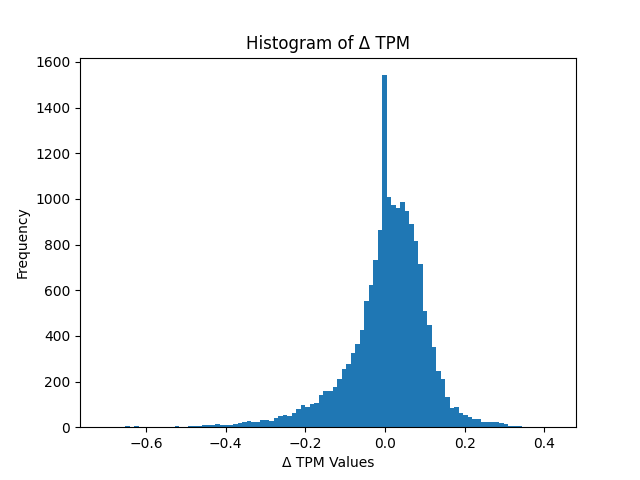
\includegraphics[width=0.5\textwidth]{figures/03_02_delta_tpm}
\caption{Distribution of $\Delta_{TPM}$ Values}
\label{fig:03_02_delta_tpm}
\end{figure}

We then define a $\Delta_{type}$ as either $increase$ or $decrease$, depending on whether the delta value is positive or negative.

As a final step for our first objective \ref{obj:delta_tpm}, we need to determine if a change in gene activity is significant. % Doppelt
To do this, we use the z score measure, which calculates how many standard deviations a delta TPM value is away
from the mean of all delta TPM values.
The $z score$ is given by:

\begin{subequations}
\begin{equation} \label{eq:z_score}
z score (x) = \frac{x - {\mu}}{\sigma}
\end{equation}
\begin{equation}
\text{where } \mu = \frac{1}{n} \sum_{i=1}^{n} x_i
\end{equation}
\begin{equation}
\text{where } \sigma = \sqrt{\frac{1}{n-1} \sum_{i=1}^{n} (x_i - \mu)^2}
\end{equation}
\end{subequations}
% TODO check formular | mean(x) = and std(x) =

where $x$ is the delta TPM value, $\mu$ is the mean of all delta TPM values, $\sigma$ is the standard deviation of all delta TPM values,

We define a threshold of  $z score = 1.96$ to indicate significant changes in gene activity,
which corresponds to a confidence level of 95\% (p = 0.05).
Genes with delta TPM values exceeding this threshold will be flagged as $true$ in the $\Delta_{tpm} relevant$ column.

The resulting table contains 17.626 Gene Nodes as rows with their associated attributes,
including TPM values and derived metrics such as Delta TPM or Z-Score.
The head of the table is shown in Figure \ref{fig:03_02_df_gene_nodes}.

\begin{figure}[h]
\centering
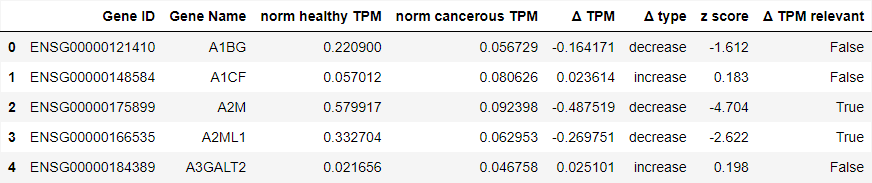
\includegraphics[height=\dfheight]{figures/03_02_gene_nodes}
\caption{Example data of Gene Nodes Table}
\label{fig:03_02_df_gene_nodes}
\end{figure}


% Gene Protein Edges
To construct the \textbf{gene-protein edges} we need a table that links the gene to the corresponding protein
which is translated from the transcript of this gene.
For this purpose we downloaded a file from biomart with Gene IDs and their Protein IDs. [LINK]
% The initial dataset comprised of XXX entries.
First we filtered for a subset (Intersection) to only include rows where the Ensembl ID for the gene matched an existing gene node
Since we have some genes without an entry for proteins, we need to drop them ; otherwise, there will not be an edge.

The final gene-protein edge table features 101,731 rows as edges and two columns:
Ensembl ID for the gene and Ensembl ID for the protein translation.
The dataset highlights a key aspect of protein biology - one gene can be translated into multiple proteins.

\begin{figure}[h]
\centering
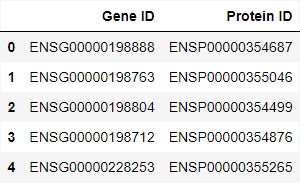
\includegraphics[height=\dfheight]{figures/03_02_gene_protein_edges}
\caption{Example data of Gene Protein Edges Table}
\label{fig:03_02_df_gene_protein_edges}
\end{figure}


% Proteins Nodes
We can generate the \textbf{protein nodes} from the gene-protein edges
since we only need a PPI for those proteins that are linked to our genes of interest.
To do this, we filter out the Gene colum from the previous file and check if there are any duplicate proteins.
Since there are no duplicate proteins our data indicates that every protein is uniquely translated by a single gene.
We do not need any additional attributes for these protein nodes because are focusing on the edges of this network.

The resulting table is a list of 101.731 unique Protein Ensembl IDs as shown in Figure \ref{fig:03_02_df_protein_nodes}.
\begin{figure}[h]
\centering
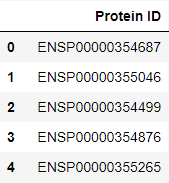
\includegraphics[height=\dfheight]{figures/03_02_protein_nodes}
\caption{Example data of Protein Nodes Table}
\label{fig:03_02_df_protein_nodes}
\end{figure}
\\

% protein protein edges
To create the \textbf{protein-protein edges} we download the String Database [LINK] with the information about the Protein Protein Interaction.
We ensure that there are no duplicate entries.

The resulting file consists of 11.247.242 rows of protein-protein edges with a column for both protein IDs for the edge.
\begin{figure}[h]
\centering
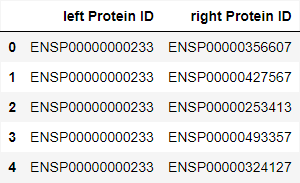
\includegraphics[height=\dfheight]{figures/03_02_protein_edges}
\caption{Example data of Protein-Protein Edges Table}
\label{fig:03_02_df_protein_edges}
\end{figure}


